\chapter{Analysis of Performance}

\section{Test Objectives}
The test campaigns presented here aim to investigate the performance of UDP communication in a local network under conditions similar to those in a distributed test support system. The considered performance indicators are latency and jitter. The investigations are performed using the star topology with the iHawk in the center, presented in \ref{chap:TopoiHawk}.

There are several factors that can contribute to the latency of a network. However, since there are no intermediate stations between the computer systems in the network topology, the focus will be on these computer systems and their operating states. In a computer system, latency is influenced by the network interface and driver, processing in the network stack, and the application.

The worst-case latency (see \ref{chap:LatencyExplanation}) is the most important indicator for these investigations. However, the mean latency should be also considered. Additionally, secondary data, such as packet losses and datagram sequence, are taken into consideration.

\section{System under Test}
Although the topology with the iHawk in the center is used, in contrast to the reliability tests with this topology (see \ref{chap:ReliabIhawk}), not all bi-directional links between the iHawk in the center and the High-Performance or Traffic PCs are to be examined simultaneously. Instead, a single isolated communication is considered.

\begin{figure}[h]
    \centering
    \begin{subfigure}[b]{0.45\textwidth}
        \centering
        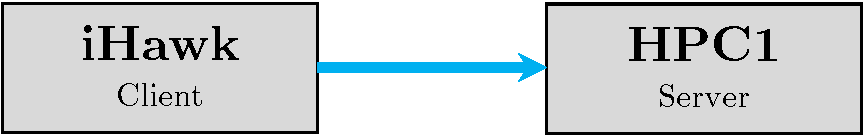
\includegraphics[width=\textwidth]{figures/performance/sut_1a.pdf}
        \caption{Direction 'H'}
        \label{fig:SutHpcPerf:H}
    \end{subfigure}
    \hfill
    \begin{subfigure}[b]{0.45\textwidth}
        \centering
        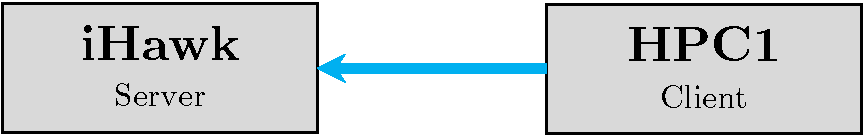
\includegraphics[width=\textwidth]{figures/performance/sut_1b.pdf}
        \caption{Direction 'R'}
        \label{fig:SutHpcPerf:R}
    \end{subfigure}
    \caption{Illustration of the used System under Test with a High-Performance PC.}
    \label{fig:SutHpcPerf}
\end{figure}

The system under test is defined as the UDP communication generated by the TestSuite. Figure  \ref{fig:SutHpcPerf} illustrates this communication between the iHawk and HPC1. Both directions are considered in the campaigns. Direction '\textbf{H}', as depicted in Figure \ref{fig:SutHpcPerf:H}, refers to the communication with iHawk as the sender and HPC1 as the receiver. In contrast, Figure \ref{fig:SutHpcPerf:R} illustrates Direction '\textbf{R}', where HPC1 acts as the sender and iHawk as the receiver.

Similarly, a UDP communication between the iHawk and TPC1 was also considered a system under test. Again, both directions were analyzed.

The network interfaces mentioned in the topology description are used unless otherwise stated in the test campaign description. Furthermore, as with the reliability tests with the iHawk in the center, several settings recommended in the Intel Linux Performance Tuning Guide for the Ethernet 700 series were used. A list of these settings can be found in chapter \ref{chap:ReliabIhawk:SuT}.

\section{Accuracy of Measurements}
As demonstrated in \ref{chap:LatencyExplanation}, latency calculation is based on the difference between two time stamps. One of them is recorded at the sender and the other at the receiver. In order to calculate a valid latency value, clock synchronization between the systems is required. The accuracy and reliability of the measurements depend on the accuracy of this clock synchronization.

The Precision Time Protocol (PTP) is utilized to synchronize clocks between the systems. PTP, as defined in IEEE 1588-2008 \cite{perf01}, synchronizes distributed clocks in a network using the master-slave principle. The master sends messages with synchronization information, enabling all slaves to synchronize their internal clocks with the master. The protocol is also able to handle time delays introduced by the network.

The programs ptp4l and phc2sys implement the PTP standard for Linux. They provide information about the accuracy of the synchronization with the master offset \cite{perf02}. Table \ref{tab:PTPMasterOffset} shows this information for the setup used in the test. HPC1 was the master and TPC1 and the iHawk were the slaves.

\begin{table}[h]
\centering
\begin{tabular}{lll}
	\toprule
	System & Role & Master Offset \\
	\midrule
 	HPC1 & Master & - \\ 
 	TPC1 & Slave & ±80 ns \\
 	iHawk & Slave & ±85 ns \\
	\bottomrule
\end{tabular}
\caption{PTP Master Offset in the Test Setup.}
\label{tab:PTPMasterOffset}
\end{table}

The data indicates that the clocks of the two slaves synchronize with the master with an accuracy of 80 to 85 ns. Since the measured latencies in the test are expected to be at least in the two- to three-digit microsecond range, the accuracy of the clock synchronization is sufficient to provide reliable latency results.

\section{Test Campaigns}









